\documentclass[a4paper, 11pt]{report}
\usepackage{blindtext}
\usepackage[T1]{fontenc}
\usepackage[utf8]{inputenc}
\usepackage{titlesec}
\usepackage{fancyhdr}
\usepackage{geometry}
\usepackage{fix-cm}
\usepackage[hidelinks]{hyperref}
\usepackage{graphicx}
\usepackage{titlesec}
\usepackage{caption}
\usepackage{subcaption}

\usepackage[english]{babel}

\geometry{ margin=30mm }
\counterwithin{subsection}{section}
\renewcommand\thesection{\arabic{section}.}
\renewcommand\thesubsection{\thesection\arabic{subsection}.}
\usepackage{tocloft}
\renewcommand{\cftchapleader}{\cftdotfill{\cftdotsep}}
\renewcommand{\cftsecleader}{\cftdotfill{\cftdotsep}}
\setlength{\cftsecindent}{2.2em}
\setlength{\cftsubsecindent}{4.2em}
\setlength{\cftsecnumwidth}{2em}
\setlength{\cftsubsecnumwidth}{2.5em}

\titlespacing\section{0pt}{12pt plus 4pt minus 2pt}{0pt plus 2pt minus 2pt}
\titlespacing\subsection{0pt}{12pt plus 4pt minus 2pt}{0pt plus 2pt minus 2pt}

\begin{document}
\titleformat{\section}
{\normalfont\fontsize{15}{0}\bfseries}{\thesection}{1em}{}
\titlespacing{\section}{0cm}{0.5cm}{0.15cm}
\titleformat{\subsection}
{\normalfont\fontsize{13}{0}\bfseries}{\thesubsection}{0.5em}{}
\titlespacing{\section}{0cm}{0.5cm}{0.15cm}

%=============================================================================

\pagenumbering{Alph}
\begin{titlepage}
\begin{flushright}

\includegraphics[width=4cm]{USyd}\\[2cm]
\end{flushright}
\center 
\textbf{\huge INFO1111: Computing 1A Professionalism}\\[0.75cm]
\textbf{\huge 2023 Semester 1}\\[2cm]
\textbf{\huge Self-Learning Report}\\[3cm]

\textbf{\huge Submission number: 3}\\[0.75cm]
\textbf{Github link: \url{https://github.com/zliu6203/SelfLearning}}\\[2cm]

{\large
\begin{tabular}{|p{0.35\textwidth}|p{0.55\textwidth}|}
	\hline
	{\bf Student name} & Zhili Liu\\
	{\bf Student ID} & 520451407\\
	{\bf Topic} & PyGame\\
	{\bf Levels already achieved} & B\\
	{\bf Levels in this report} & D\\
	\hline
\end{tabular}
}
\thispagestyle{empty}
\end{titlepage}
\pagenumbering{arabic}


%=============================================================================

\tableofcontents

%=============================================================================

\newpage
\section*{Instructions}

\textbf{Important}: This section should be removed prior to submission.

You should use this \LaTeX\ template to generate your self-learning report. Keep in mind the following key points:
\begin{itemize}
	\item \textbf{Submissions}: There will be three opportunities during the semester to submit this report. For each submission you can attempt 1 or 2 levels. Each submission should use the same report, but amended to include new information.
	\item \textbf{Assessment}: In order to achieve level B, you must first have achieved level A, and so on for each level up to level D. This means that we will not assess a higher level until a lower level has been achieved (though we will review one level higher and give you feedback to help you in refining your work).
	\item \textbf{Minimum requirement}: Remember that in order to pass the unit, you must achieve at least level A in the self-learning (unless you achieve level B in both the skills and knowledge categories).
	\item \textbf{Using this template}: When completing each section you should remove the explanation text and replace it with your material.
	\item \textbf{Referencing}: You should also ensure that any resources you use are suitably referenced, and references are included into the reference list at the end of this document. You should use the IEEE reference style \cite{usyd2} (the reference included here shows you how this can be easily achieved).
\end{itemize}


%=============================================================================


\newpage
\section{Level A: Initial Understanding}
\vspace{5mm}
\subsection{Level A Demonstration}
The three things that demonstrate my understanding for this topic are:
\begin{itemize}
	\item Make a successful window for PyGame including some screen elements (sprites).
	\item Using sound libraries.
	\item Responding to user input.
\end{itemize}

\subsection{Learning Approach}
I approached my learning by looking for the latest tutorials online with PyGame, specifically the ones with project examples. I browsed both video and website tutorials including official documentation for many new methods and modules to build a successful game using the PyGame module of Python.

Experimentation was my main method of learning; testing all the different built-in libraries of methods and objects including sprites ("draw" module), sounds ("mixer" module), and the window itself ("display" module). I self-learnt by using previous knowledge of game development in C\# and Java to my advantage - scenes, object priority, using external files etc. Additionally, I also used knowledge of window composition via WinForms and Tkinter.

\subsection{Challenges and Difficulties}
Due to the new syntax it was difficult to correctly load a window at all with the limited knowledge. The most difficult to learn was the while loop that the game is running on; it also contains a for loop which did not make much sense. I simply accepted it as fact instead of fully understanding it.

Even after the window was created, it was even more difficult to find any sprites to fill the window as opposed to Tkinter or WinForms, where sprites and screen elements were ready for use. Furthermore, PyGame did not include any built-in sound files and so sound effects \& music must be found online or created locally.


\subsection{Learning Sources}
\begin{tabular}{|p{0.45\textwidth}|p{0.45\textwidth}|}
	\hline
	Learning Source & Contribution to Learning\\
	\hline
	\href{https://www.pygame.org/wiki/tutorials}{Wiki tutorial} & Understanding what each module does and its methods and objects.\\
	\hline
	\href{https://www.youtube.com/watch?v=jO6qQDNa2UY}{Beginner video tutorial} & Understanding the basics of every major aspect of PyGame.\\
	\hline
	\href{https://www.pygame.org/docs/ref/mouse.html}{Official documentation (mouse input)} & Finding each method and the parameters necessary for these methods.\\
	\hline
	\href{https://opensource.com/article/20/9/add-sound-python-game}{Sound help} & Understanding how sound works and how to implement sound at an appropriate time.\\
	\hline
	\href{https://www.youtube.com/watch?v=YDP1Hk7uZFAs}{Another video tutorial for shapes} & Understanding what to do in the absence of assets with sprites.\\
	\hline
\end{tabular}
\\
\\
\subsection{Application artifacts}
In level A, I made a very simple program in PyGame demonstrating that a successful window (1280x720) is opened with some screen elements (background, red line, blue player square). The blue square is responding to user input by following the coordinates of the mouse and not allow the mouse to go past the red line or the screen. When the cube touches the red line, a sound effect is played exactly once. This is demonstrated in this diagram.

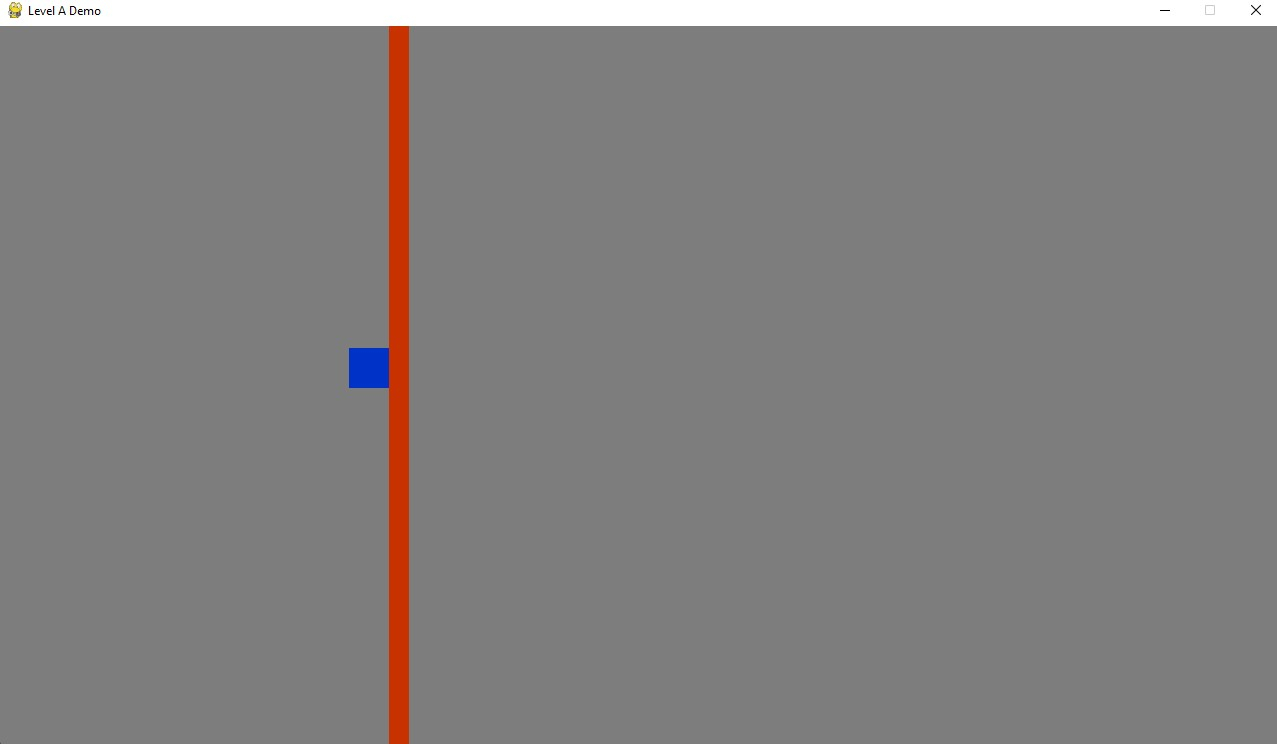
\includegraphics[width=8cm]{Level A Demo}\\[1cm]
\\
In the code, I used simple python syntax with some new PyGame methods and elements. In the follwing screengrabs, I showed this by using the main function and setting initial variables.

\begin{figure}[!htb]%
    \centering
    \subfloat[\centering Code showing variables]{{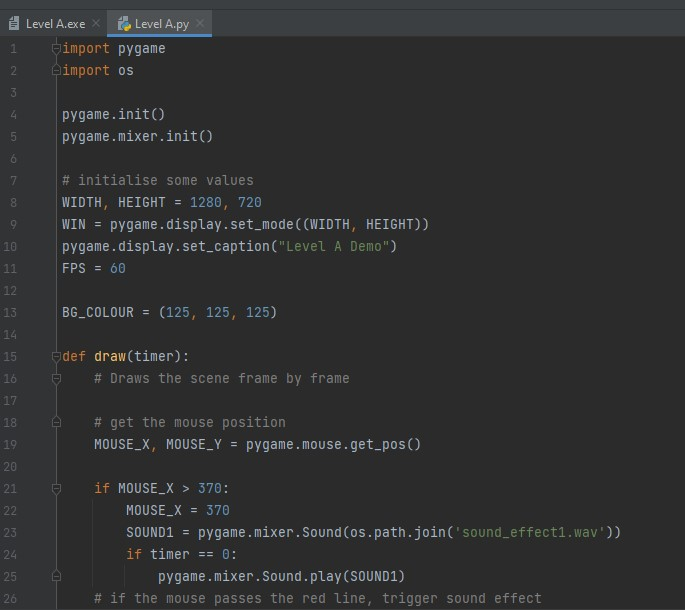
\includegraphics[width=6.5cm]{Level A Demo Code1} }}%
    \qquad
    \subfloat[\centering Code showing main function]{{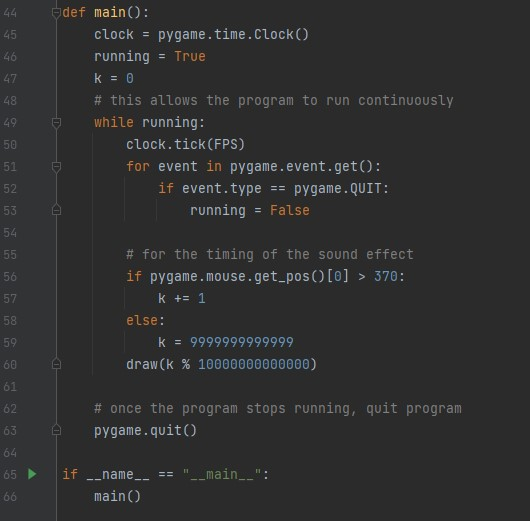
\includegraphics[width=6.5cm]{Level A Demo Code2} }}%
\end{figure}

Additionally, I used a simple sound effect from the web (sound\_effect1.wav) to play whenever the player hits the red line. I also used pyinstaller to make the .py into a .exe which is also included in the Git repository.

%=============================================================================

\newpage
\section{Level B: Basic Application}

Whilst level A is about doing something simple with the topic to just show that you have started to be able to use the tool or technology, level B is about doing something practical that might actually be useful.

\subsection{Level B Demonstration}

The application I have developed is a simple game in PyGame. This involves the three points in the level B proposal: events such as scenes, making a simple game with an end goal (win/lose), and program simple enemies. I have demonstrated the first point by making different levels in the game, satisfied the second point by creating a game with a goal (to finish all 5 levels), and also programmed simple enemies with random movement and bouncing back from the screen if it goes offscreen.

\subsection{Application artifacts}

I have created a simple topdown shooter game using built-in assets, modules, and tools only. The game I have made is simple: shoot all enemies using a periodic laser which can destroy all enemies collided with the laser. I used classes and small aspects of object oriented programming to achieve this.

In the following screengrab, the player can shoot a laser which only fires when the left mouse button is pressed and the cooldown for the laser is done. This laser collides with all enemies within its vicinity and destroys them. The player in blue and white can be controlled using WASD and the laser is shot in the direction of the cursor.
\\
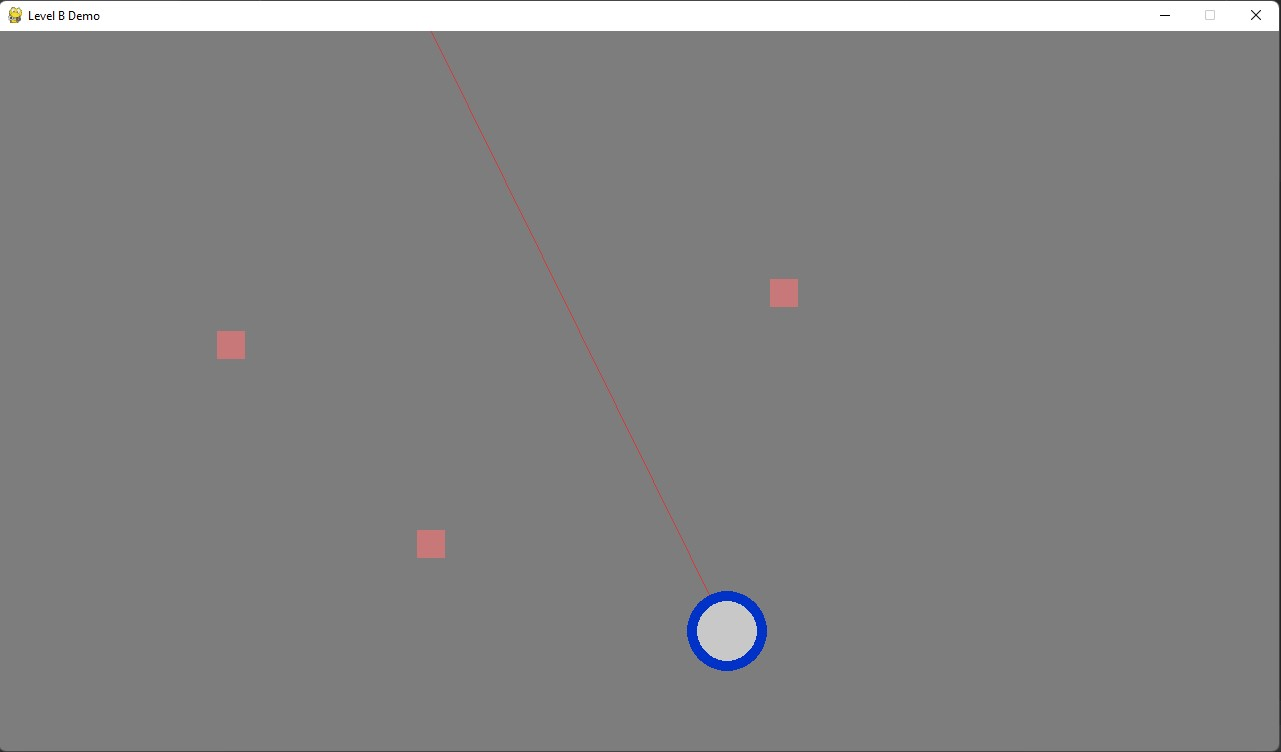
\includegraphics[width=8cm]{Level B Demo}\\[1cm]
\\

This screengrab shows the huge number of enemies in level 4 of this game:
\\
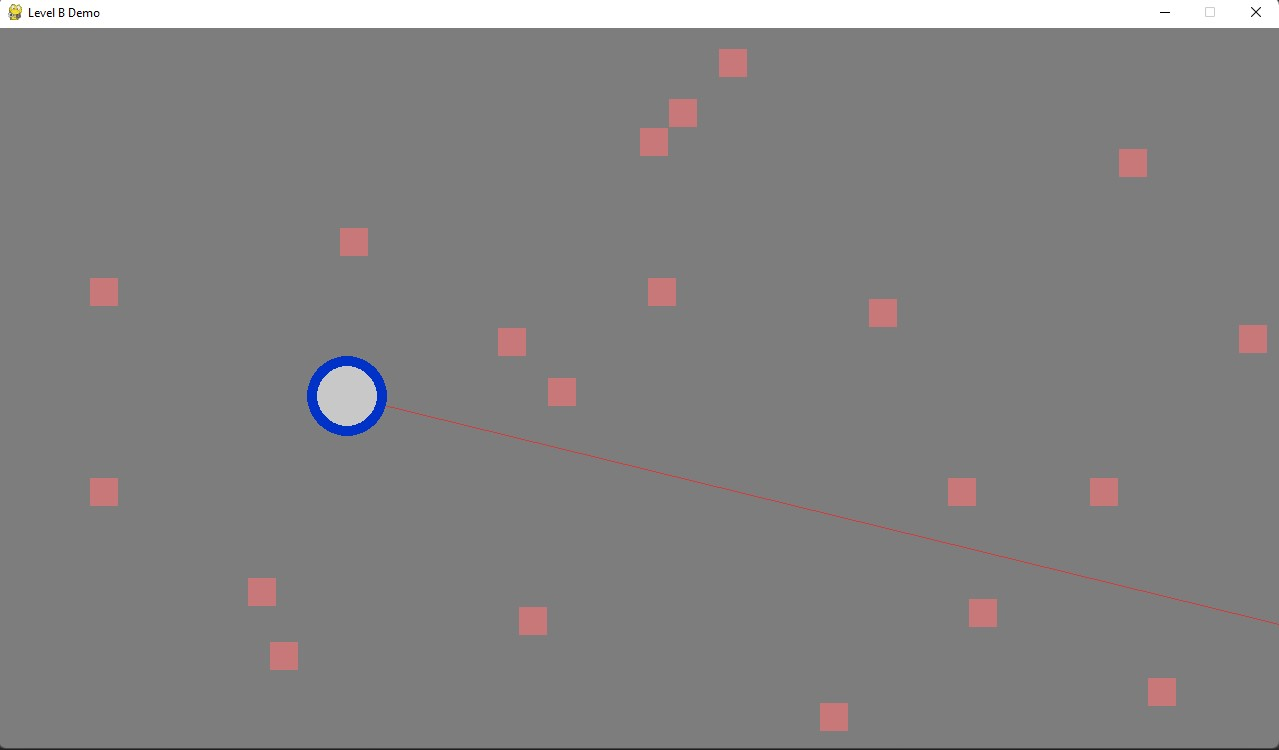
\includegraphics[width=8cm]{Level B Demo2}\\[1cm]
\\
This code snippet shows the object oriented programming and the hierarchy of classes and objects. The Entity class includes both the Player and Enemy classes as its children. The enemy class also contains code for random movement (see more in GitHub).

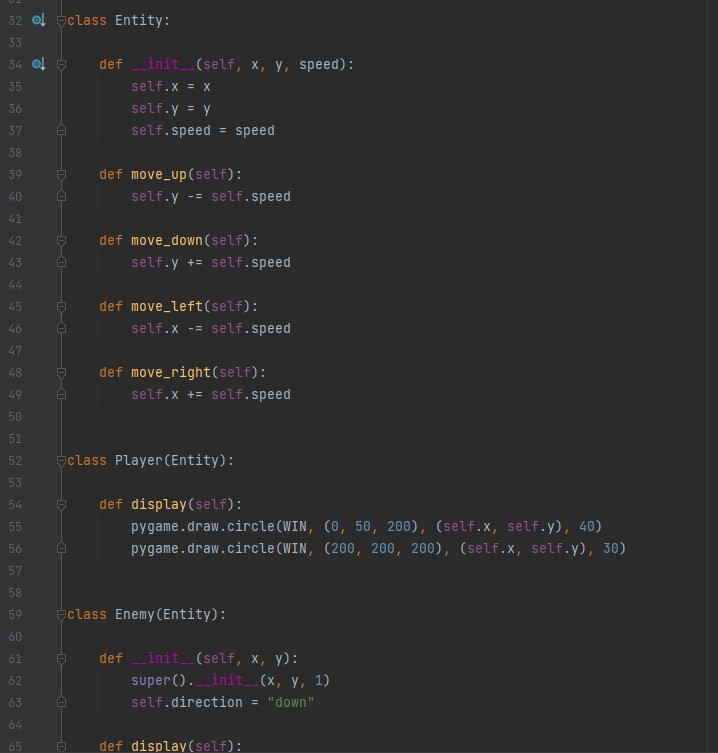
\includegraphics[width=8cm]{Level B Demo Code1}\\[1cm]
\\

These two code snippets shows the Game class being the main class which handles all the events.

\begin{figure}[!htb]%
    \centering
    \subfloat[\centering Code showing Game class]{{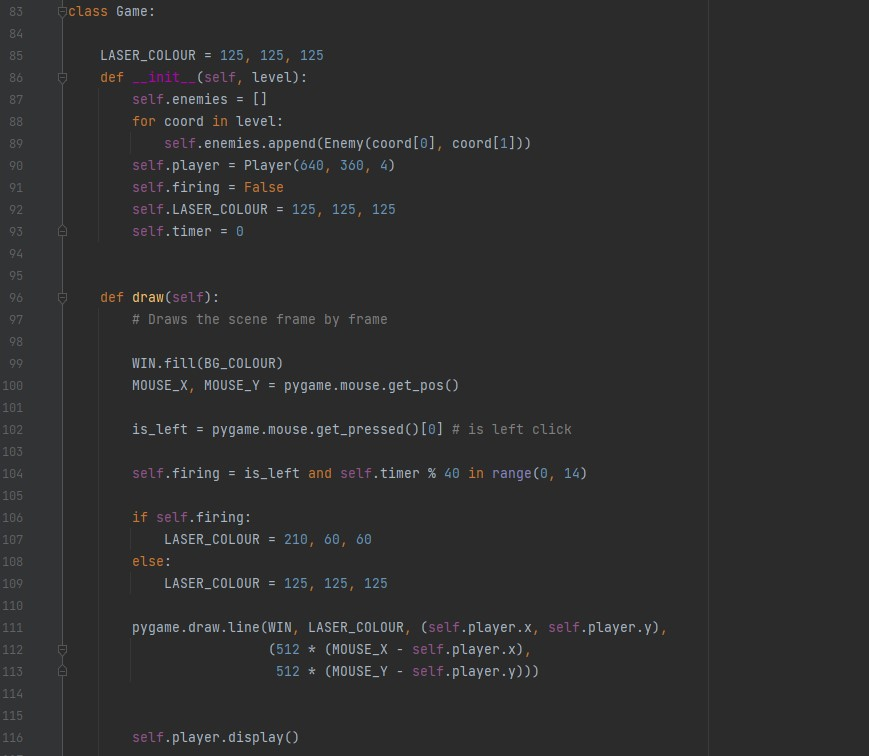
\includegraphics[width=6.5cm]{Level B Demo Code2} }}%
    \qquad
    \subfloat[\centering Code showing how enemies work]{{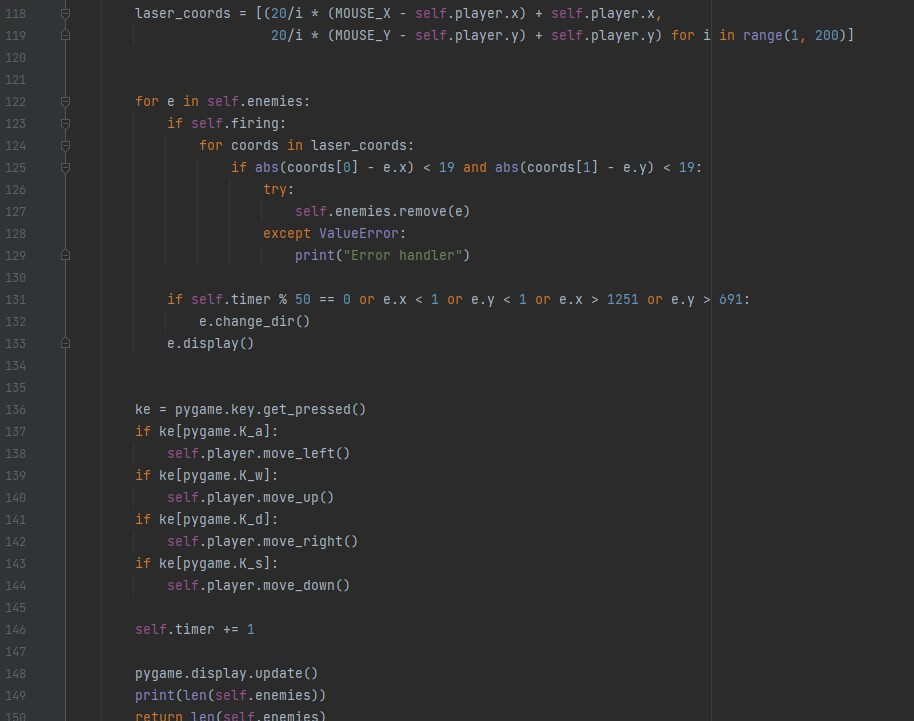
\includegraphics[width=6.5cm]{Level B Demo Code3} }}%
\end{figure}


%=============================================================================

\newpage
\section{Level C: Deeper Understanding}

Level C focuses on showing that you have actually understood the tool or technology at a relatively advanced level. You will need to compare it to alternatives, identifying key strengths and weaknesses, and the areas where this tool is most effective. 

\subsection{Strengths}
Python is an easy language to learn and PyGame is very lightweight (i.e., takes up little memory). PyGame can be a valuable introduction to game development as it allows beginners to learn the fundamentals of graphics programming, manipulating the GUI, interactivity, using sound and music libraries, and many more. Furthermore, PyGame excels at implementing simple functionalities using much less code than alternatives such as Unity or Unreal Engine, for example collisions and player input \cite{pygame_pros}. The PyGame community has plenty of sprites and sound files to choose from so the programmer does not need to make them from scratch.

\subsection{Weaknesses}
PyGame contains limited features as well as lacking in speed when compared to alternatives. The Python language is generally much slower and more minimalistic than other C based languages including Java, C\#, and C++, the latter two are what Unity and Unreal Engine are based on. As such, PyGame syntax can be very confusing for more complex mechanics such as firing projectiles or implementing physics. PyGame is also “semi-portable” as distribution onto different platforms requires a native version of PyGame \cite{pygame_cons}, in addition to being difficult to distribute due to Python’s syntax, which are major inconveniences.  

\subsection{Usefulness}
PyGame is useful for developing small games in a short period of time as Python is very efficient at executing simple tasks \cite{pygame_uses}. One scenario is where an experienced game programmer or team comes up with an original idea for a game; instead of building the game directly, they can use PyGame to create a fast and simple design (as a planning phase) to spot potential loopholes and development issues. PyGame can be used as a tool for designing and testing more advanced game ideas using other engines simply due to how rapid the development can be.

\subsection{Key Question 1 - Is PyGame useful for 3D First Person games? Or only 2D games?}
PyGame itself is only useful for 2D games due to a lack of physics engines, rendering software, and using 3D models and environments. PyGame can handle basic 3D graphics but that is done with incredibly long and complex code, while also being very slow. Furthermore, as discussed earlier, it is difficult to distribute the completed software, making it even less ideal to package 3D games. However, with the introduction of other modules such as PyOpenSQL and PyGlet to form PyEngine3D \cite{pygame_3d}, it is much more viable to create simple 3D games, many of which can be found in the community. However, it is observed that very few are first person 3D games, which shows the complexity of this task.

\subsection{Key Question 2 - How good a Python programmer do you need to be before you can use PyGame effectively?}
PyGame, much like every other game engine, require a solid knowledge of objects, methods, modules and data from the parent language (Python) to create effective games. High-level control systems, such as the ones mentioned before, are needed to allow the developed game to be interactive and responsive to input. An understanding of classes and methods allows manipulation of one group of objects and easy replication of features (e.g., enemy or game structure). Moreover, other modules and using data is important for distribution of software, allow variability from other projects (promotes original ideas), and most importantly saving information to a local or online database for future access.\cite{pygame_python}


%=============================================================================

\newpage
\section{Level D: Evolution of skills}
\vspace{5mm}
\subsection{Level D Demonstration}

I have developed a simple top-down shooter game where the goal is to clear a level of all enemies before moving on. In total there are 5 levels and 5 different types of enemies with their own unique abilities. The player controls a laser (space or mouse click) which can decrease the health of any enemies in contact with them. The game contains a main menu, as well as screens for victory, game over and level clear (see below). To run the program from GitHub, run the "level\_D.exe" file provided (does not work with Mac).

\subsection{Application artifacts}

The actual application developed from PyGame is a .exe file generated from "auto-py-to-exe", much like level A:
\begin{figure}[h]
    \centering
    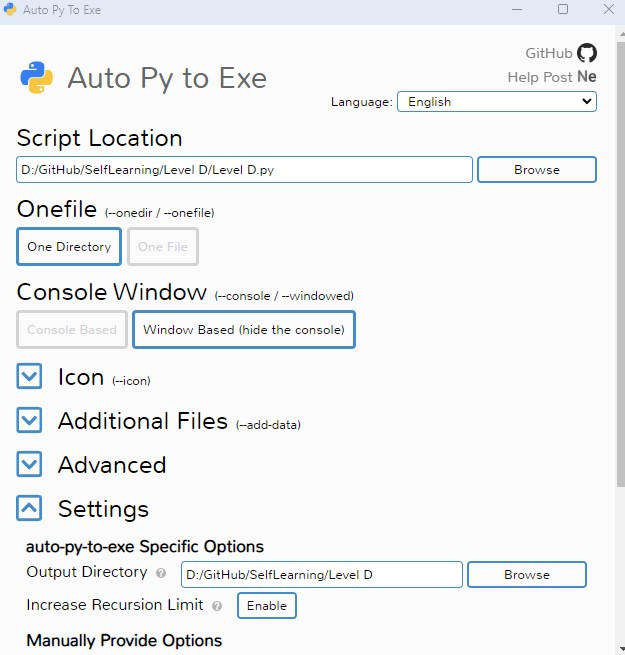
\includegraphics[width=\textwidth]{auto-py-to-exe}
    \caption{Using level D python file and the directory contents to convert to exe file.}
\end{figure}
\\\\
When opened, the game greets the player with a menu screen, generated from the Menu class. This is always the first thing executed when main() is run, which makes it useful for replaying a game-over or victory:
\begin{figure}[h]
    \centering
    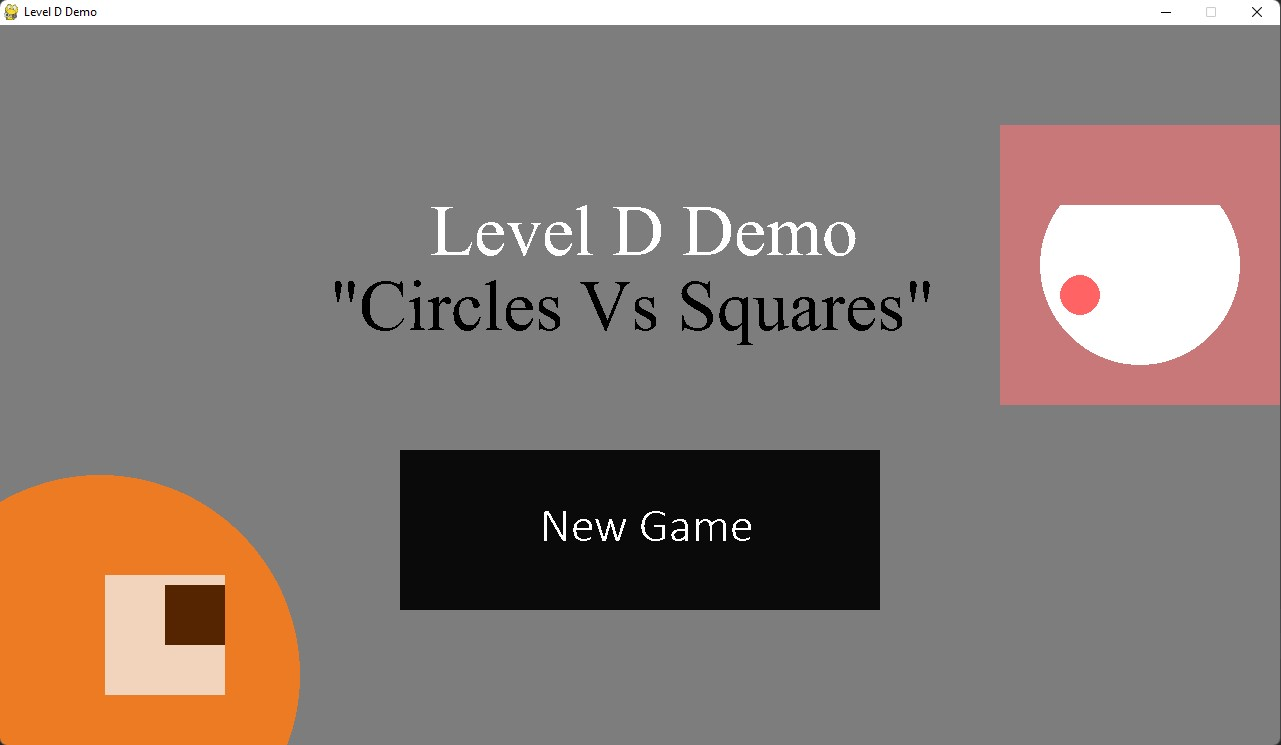
\includegraphics[width=0.8\textwidth]{mainmenu}
    \caption{Main menu, "New Game" button turns gray when highlighted.}
\end{figure}
\begin{figure}[h]
    \centering
    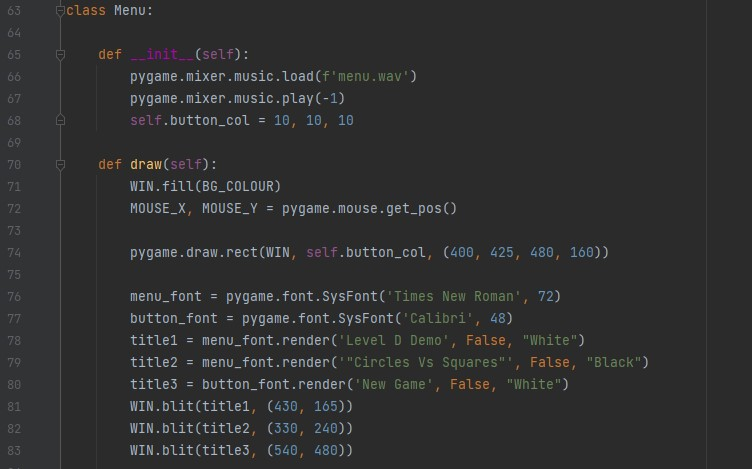
\includegraphics[width=0.8\textwidth]{menu_code}
    \caption{Menu class}
\end{figure}
\\
Furthermore, the user will also experience multiple music tracks and sound effects in the playthrough. These sounds are used from freesound.org \cite{freesound} as they are copyright free. How the music and SFX were implemented was based solely off of the official PyGame docs website \cite{pygame_mixer}. Some sounds were manipulated in FL Studio for EQ - making the game volume consistent as some sounds were much louder than others.
\\\\\\\\\\

\begin{figure}[h]
    \centering
    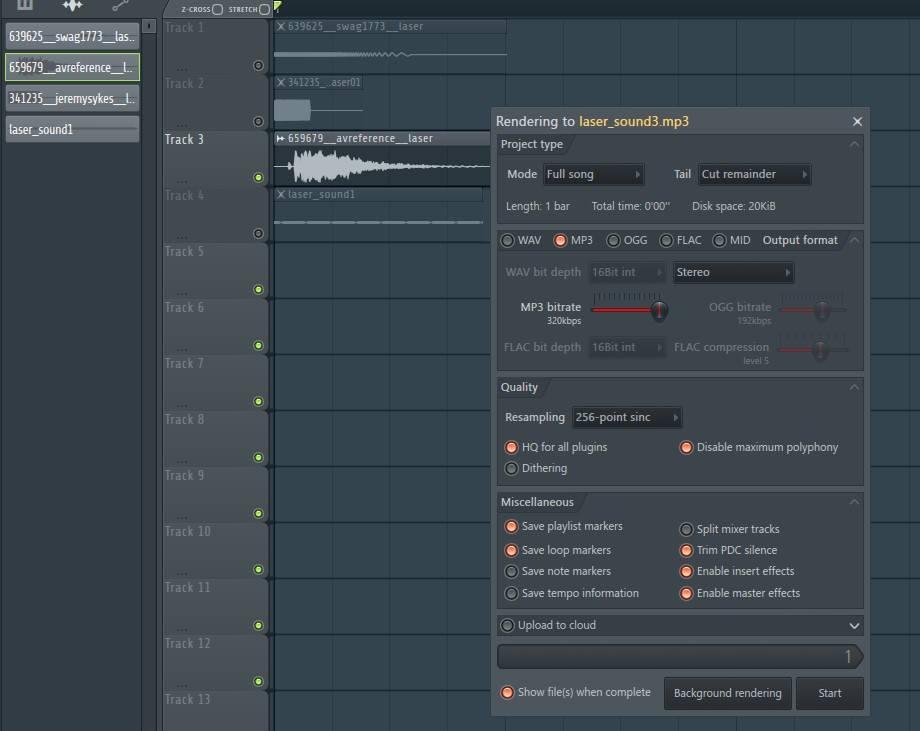
\includegraphics[width=0.6\textwidth]{flstudio}
    \caption{The use of FL Studio to balance gain or volume of music/sound effects.}
\end{figure}
\begin{figure}[h]
    \centering
    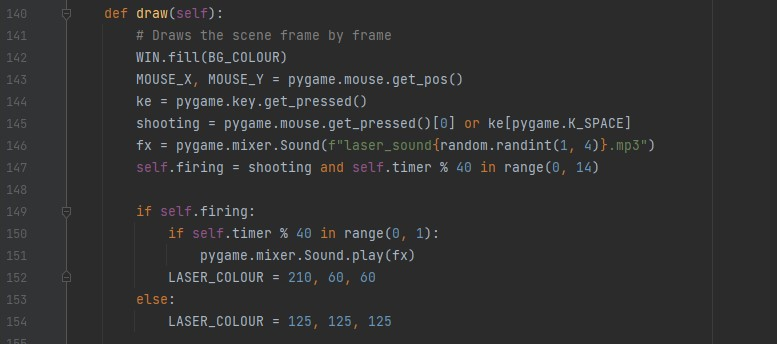
\includegraphics[width=0.8\textwidth]{shootingsound}
    \caption{Implementation of the randomised shooting sound heard in-game.}
\end{figure}
When the game starts, every level contains its own music and "waves", which are set swarms of enemies defined by multiple csv files (comma separated values). The numbers shown in figure 8 represents how many of a particular type of enemy is to be spawned. Each row is one wave of enemy, so level 5 has 7 waves of enemies. Note that these csv files only define the number and types of enemies spawned in a wave/level and not their spawn location.
The spawn location is instead defined by the function "enemy\_spawn" which returns a list of random coordinates outside of the screen. Enemies move much fast and are invincible outside the screen (figure 9).
\\\\\\\\\\\\\\\\\\\\\\\\

\begin{figure}[h]
    \centering
    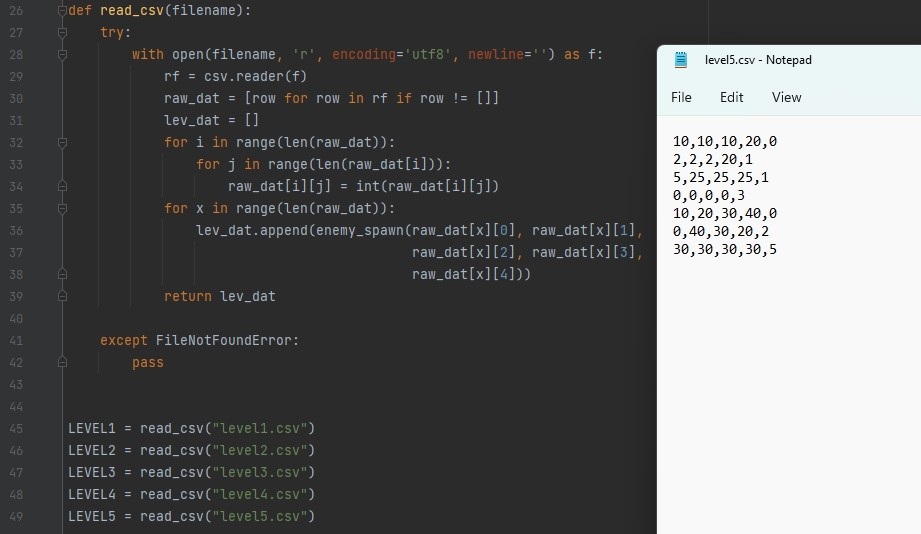
\includegraphics[width=0.8\textwidth]{csv}
    \caption{Csv module in Python and working with csv files.}
\end{figure}
\begin{figure}[h]
    \centering
    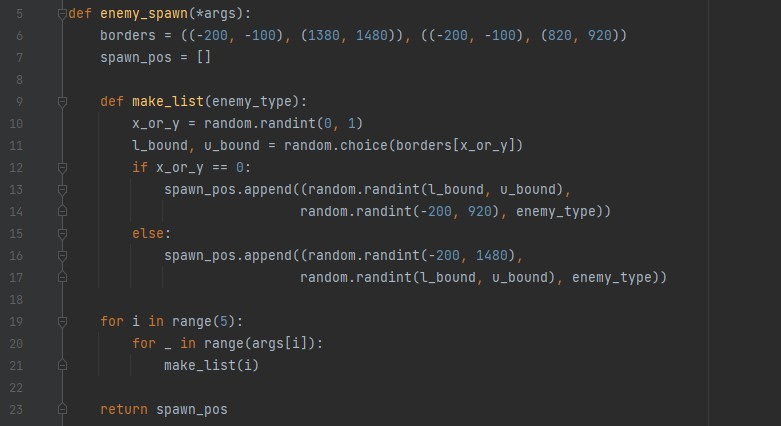
\includegraphics[width=0.8\textwidth]{random_spawn}
    \caption{Function which randomises enemy spawn coordinates.}
\end{figure}
There are five different enemies implemented:
\begin{itemize}
  \item NormalEnemy - enemy with average health and speed (green)
  \item FastEnemy - enemy with low health and fast speed (red)
  \item TankyEnemy - enemy with high health and low speed (blue)
  \item RegenEnemy - enemy with average health and speed but regenerates health (magenta)
  \item BossEnemy - enemy which has the properties of all enemies (i.e., fast, tanky, and regenerates health) (black)
\end{itemize}

Each enemy has their own class which are children of the Enemy class, which is in turn a child of the Entity class. This class structure was explained level B. Each enemy's unique sprites were made by trial and error - adjusting the sprite depending on observation in game.

Enemies show their health bar when their health is not full. This also applies for the player. BossEnemy removes more health than all other enemies, making them dangerous. All classes and objects (except Game and Menu) are defined in another file called "objects.py".

Some gameplay and code for enemies are shown:
\\
\\
\\\\\\
\begin{figure}[h]
    \centering
    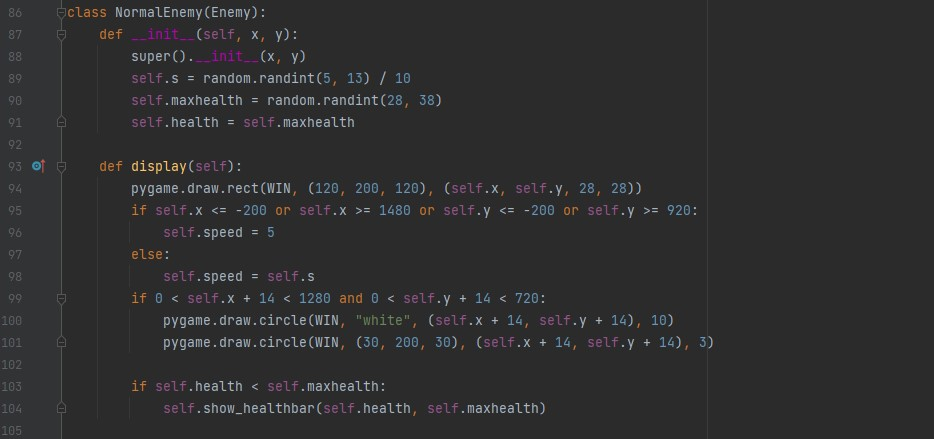
\includegraphics[width=0.8\textwidth]{normal_enemy}
    \caption{Class NormalEnemy has all properties of the green enemy}
\end{figure}
\begin{figure}[h]
    \centering
    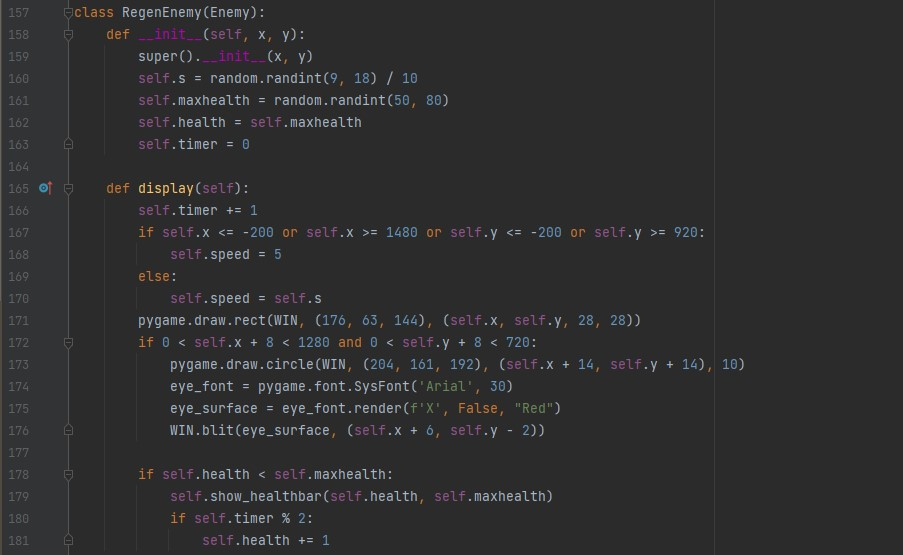
\includegraphics[width=0.8\textwidth]{regen_enemy}
    \caption{Class RegenEnemy allows the enemy to possess regeneration.}
\end{figure}

\begin{figure}[h]
    \centering
    \includegraphics[width=0.8\textwidth]{level4-5}
    \caption{Screenshot of TankyEnemy (blue), RegenEnemy (magenta) and BossEnemy (black).}
\end{figure}


\newpage
\newpage
\subsection{Alternative tools/technologies}
Unreal Engine and Unity
\subsection{Comparative Analysis}
Unity is both a 3D and 2D game engine capable of producing high quality end-products. Like Unreal Engine, it is a multi-platform tool written in C languages. PyGame does not natively support 3D engines, but 2D games are much easier to conceptualise and develop in PyGame or Unity due to the simple tool set available (only python is needed to learn PyGame whereas extensive software knowledge is needed for both engines). As such, PyGame excels at designing quick-and-easy solutions, in addition to less computing power and memory/storage.\cite{unity_pygame}

However, PyGame lacks the continual community support and frequent updates unlike Unreal Engine, which, despite its complexity, generates much better graphics and rendering technologies compared to even Unity. Unreal Engine allows development of quality games commonly seen in the commercial market, whereas Unity sees less due to less advanced graphics handling.\cite{unity_unreal}

Ultimately, efficiency and simplicity is PyGame's best features, but it lacks complexity and 3D handling; Unreal Engine contain high quality features but it is difficult to learn and usually requires teams of programmers/graphic designers; Unity also contain high quality features AND workable alone, but it is relatively difficult to learn compared to PyGame and less graphic-intensive than Unreal Engine.

%=============================================================================

\newpage
\bibliographystyle{ieeetran}
\bibliography{main}

\end{document}
\end{report}
